
\section{Experimental Analysis}

We study a dataset of news events gathered from news headlines from a
\emph{manually curated} list of well-known news media accounts (e.g., @CNN,
@BreakingNews, @BBCNews, etc.) in the microblogging platform
Twitter~\cite{twitter}.
%
Headlines were collected periodically every hour, over the course of
approximately one year. 
%
In parallel, all the Twitter messages were extracted for each news event using
the public API \cite{twitterapi}.
%
This process was performed by automatically extracting descriptive sets of
keywords for each event using a variation of frequent itemset
extraction~\cite{Tan_Steinbach_Kumar} over the event's headlines. 
%
These sets of keywords were then used to retrieve corresponding user tweets for
each event. 
%
We validate the events gathered in our data collection process to ensure that
each group of social media posts corresponds to a meaningful and cohesive news
event. 
%
We provide a detailed description of the collection methodology and of
the validation of event cohesiveness in Chapter~\ref{chapter:data}.
%
Overall, the resulting dataset contains $43,256,261$ tweets that account for
$5,234$ events (Table~\ref{table:hi:dataset-stats}).


\begin{table}
  \centering
  \begin{tabularx}{\textwidth}{@{}p{6cm}llll@{}}
    \toprule
    \textbf{News events' property} & \textbf{Minimum} & \textbf{Mean} & \textbf{Median} & \textbf{Maximum} \\ \midrule
    \# of posts & 1,000 & 8,254 & 2,474 & 510,920 \\
    \# of keywords & 2 & 3.77 & 3 & 39 \\
    Event duration (hours) & 0.12 & 20.93 & 7.46 & 190.43 \\ \bottomrule
  \end{tabularx}
  \caption{High-level description of the dataset of news events.} 
  \label{table:hi:dataset-stats}
\end{table}



In Figure~\ref{fig:hi:components} we characterize an example event from our
dataset, by showing the set of keywords and a sample of tweets associated to the
event. 
%
These keywords form a semantically meaningful event; they refer to the incident
where soccer player Luis Suarez was charged for biting another player during the
FIFA World Cup in 2014. 
%
This general collection process results in a set of social media posts
associated to an event which can encompass several memes, viral tweets and
pieces of information. 
%
Therefore, an event is composed of diverse information, addressing more
heterogeneous content than prior
work~\cite{Castillo:2014,Szabo:2010,Lerman:2010,Tatar:2011,Pinto:2013,Ahmed:2013,suh2010want}
which focus on single pieces of information (e.g., a particular meme, a viral
tweet etc.).


\begin{figure}
  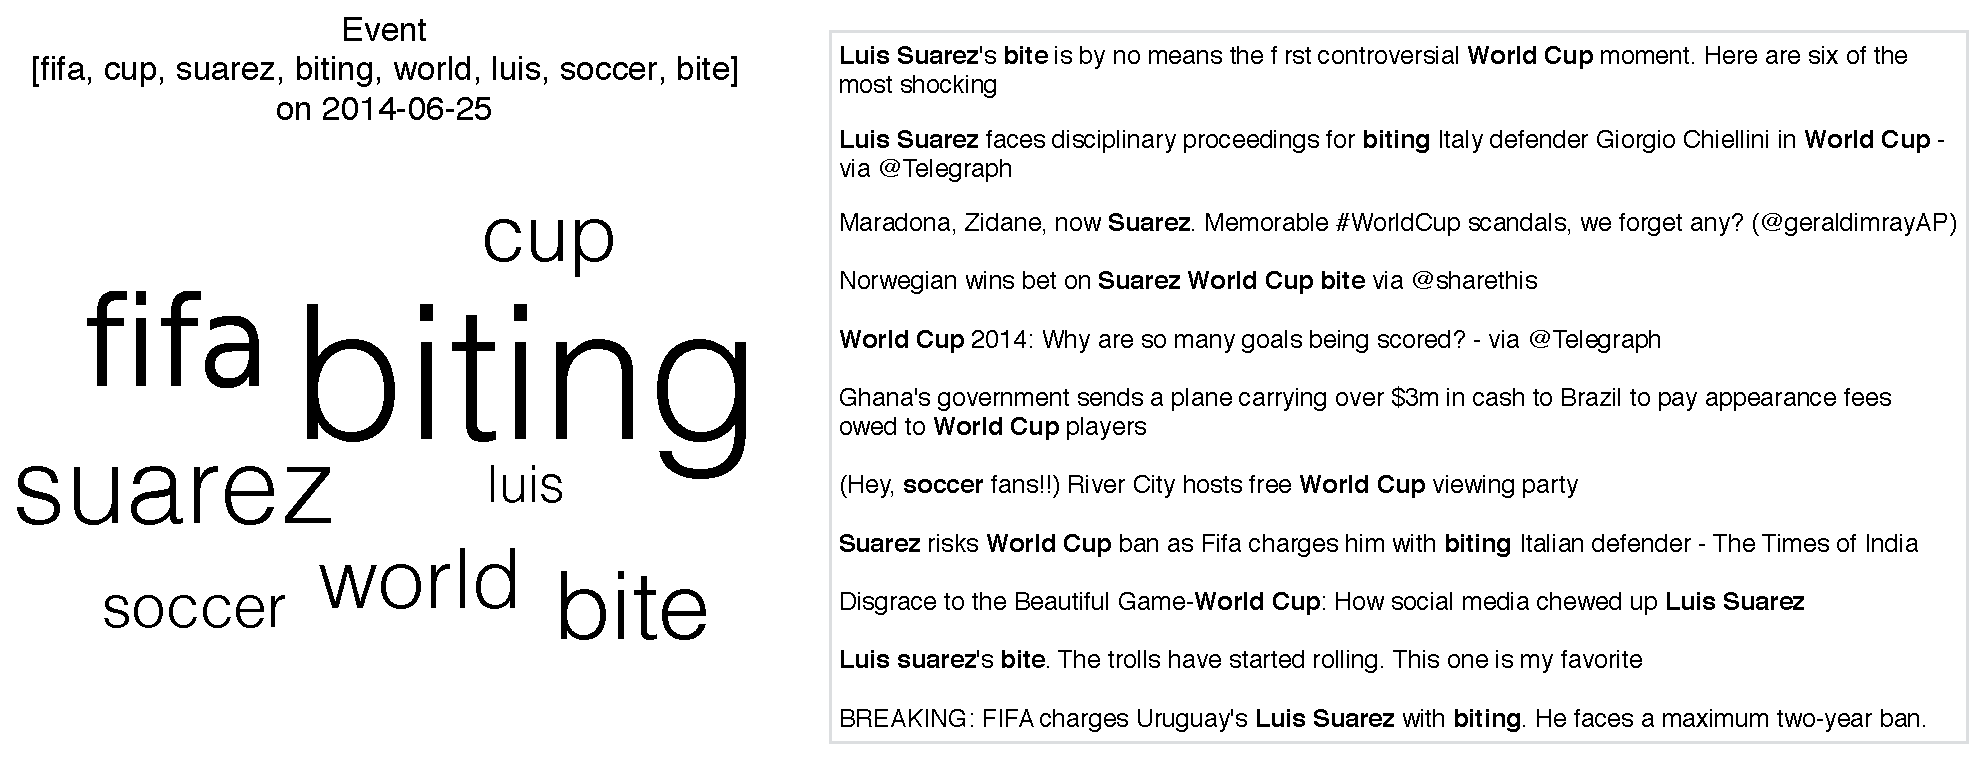
\includegraphics[width=\textwidth]{figures/high-activity/fig2}
  \caption[Example event]{A representative event, collected on 2014-06-25 with
      keywords (left) and sample user posts (right) collected from the Twitter
      Search API. Collected user posts contain at least one pair of keywords. }
  \label{fig:hi:components}
\end{figure}


The collection of events is converted into their VQ-event model representation. 
%
Using this model, we can identify events that have produced similar levels of
activity in the social network. 
%
In other words, events are considered to have similar activity if the
inter-arrival times between their social media posts are similarly distributed,
implying a very much alike collective reaction from users to the events within a
group. 
%
In order to identify groups of similar events, we cluster the event models. 
%
We sort the resulting groups of events from highest to lowest activity,
according to the concentration of social media posts in the bins that correspond
to short inter-arrival times. 
%
We consider the events that fall in the top cluster to be high-activity events
as most of their inter-arrival times are concentrated in the smallest interval of
the VQ-event model.
%
In our dataset, these correspond to roughly 8\% of the events. 
%
We consider the next clusters in the sorted ranking to form medium-high activity
events, and so on. 
%
Thus we end with four groups of events: high, medium-high, medium-low and low.
Figure~\ref{fig:hi:heatmap} shows a heatmap of the inter-arrival relative
frequency for each cluster. 
%
This classification of events based on activity intensity is independent of
event size. 


\begin{figure}
  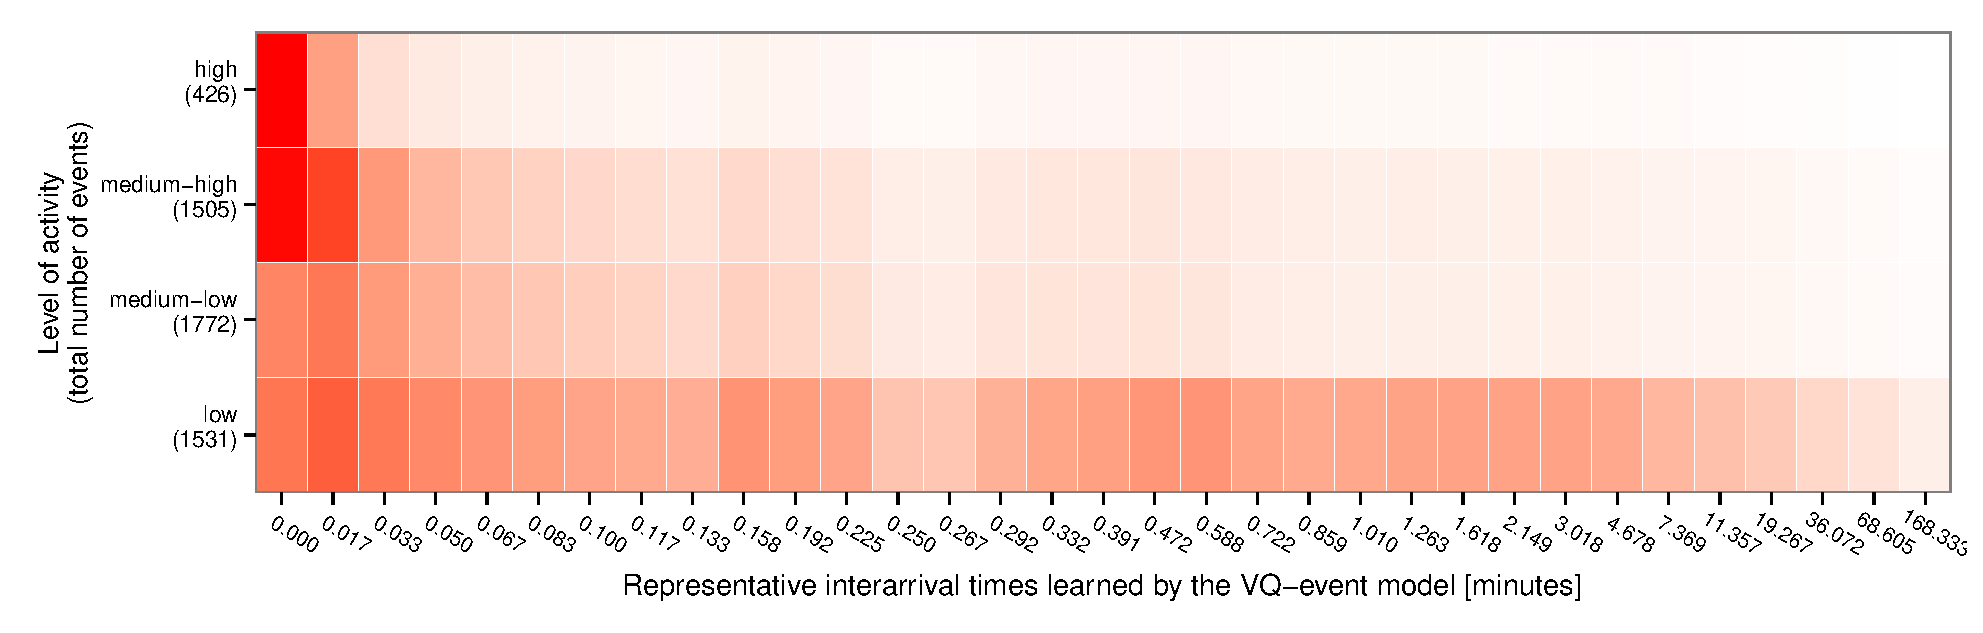
\includegraphics[width=\textwidth]{figures/high-activity/fig3}
  \caption[Heatmap of the categorization of events into clusters of
  activity.]{{Heatmap of the categorization of events into clusters of activity.
  Each row is the average representation of all the events in that clusters.  A
  darker cell represents a higher value. The y-axis specifies the number of
  events in that cluster. Clusters are (top to bottom): high-impact,
  medium-high, medium-low, and low.}}
  \label{fig:hi:heatmap}
\end{figure}